\documentclass[12pt]{article}
% Chinese Support
\usepackage{xeCJK}
\setCJKmainfont{STSong}
% \setmainfont{Times New Roman}


% for symbol
\usepackage{gensymb}
% matrix
\usepackage{amsmath}


% For images
\usepackage{graphicx}
\graphicspath{ {./screenshoot/} }

\newcommand{\numpy}{{\tt numpy}}    % tt font for numpy

\topmargin -1.in
\textheight 9in
\oddsidemargin -.25in
\evensidemargin -.25in
\textwidth 7in


\usepackage{listings}
\usepackage{color}

\definecolor{dkgreen}{rgb}{0,0.6,0}
\definecolor{gray}{rgb}{0.5,0.5,0.5}
\definecolor{mauve}{rgb}{0.58,0,0.82}

\setmonofont{FiraCode-Regular}
\lstset{frame=tb,
  language=C++,
  aboveskip=3mm,
  belowskip=3mm,
  showstringspaces=false,
  columns=flexible,
  basicstyle={\small\ttfamily},
  numbers=none,
  numberstyle=\tiny\color{gray},
  keywordstyle=\color{blue},
  commentstyle=\color{dkgreen},
  stringstyle=\color{mauve},
  breaklines=true,
  breakatwhitespace=true,
  tabsize=3
}



% Content start below
\begin{document}

\author{陈铭涛\\16340024}
\title{计算机图形学 Homework 5 - Camera}
% \date{\vspace{-5ex}}
\maketitle

\medskip

% ========== Begin answering questions here

\section{Basic}

\begin{enumerate}
    \item 投影(Projection)
    \begin{enumerate}
        \item 正交投影(orthographic projection):实现正交投影,使用多组(left, right, bottom, top, near, far)参数, 比较结果差异
        
        正交投影使用了如下的平截头体进行裁剪:
        \begin{center}
            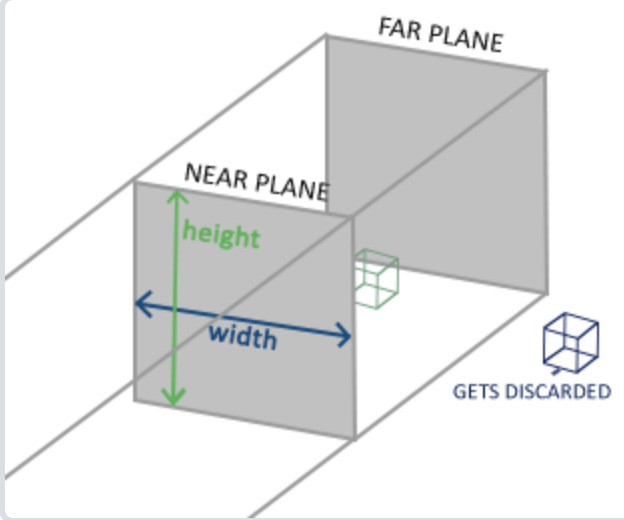
\includegraphics[scale=0.5]{ortho_img.png}
        \end{center}
        
        使用 GLM 库的 ortho 函数实现,其函数签名如下:
        \begin{lstlisting}
detail::tmat4x4<T> glm::gtc::matrix_transform::ortho(
        T const &   left,
		T const &  	right,
		T const &  	bottom,
		T const &  	top,
		T const &  	zNear,
		T const &  	zFar 
) 	
        \end{lstlisting}
        其中,left 和 right 参数表示正交投影平截头体的左右坐标,bottom 和 top 参数代表上下坐标,zNear 和 zFar 则是近平面和远平面的距离。

        正交投影将把所有坐标映射到2D 的屏幕中,但是可能会产生不真实的结果,将cube放置在(-1.5, 0.5, -1.5)位置后通过正交投影获得的结果如下:
        \begin{center}
            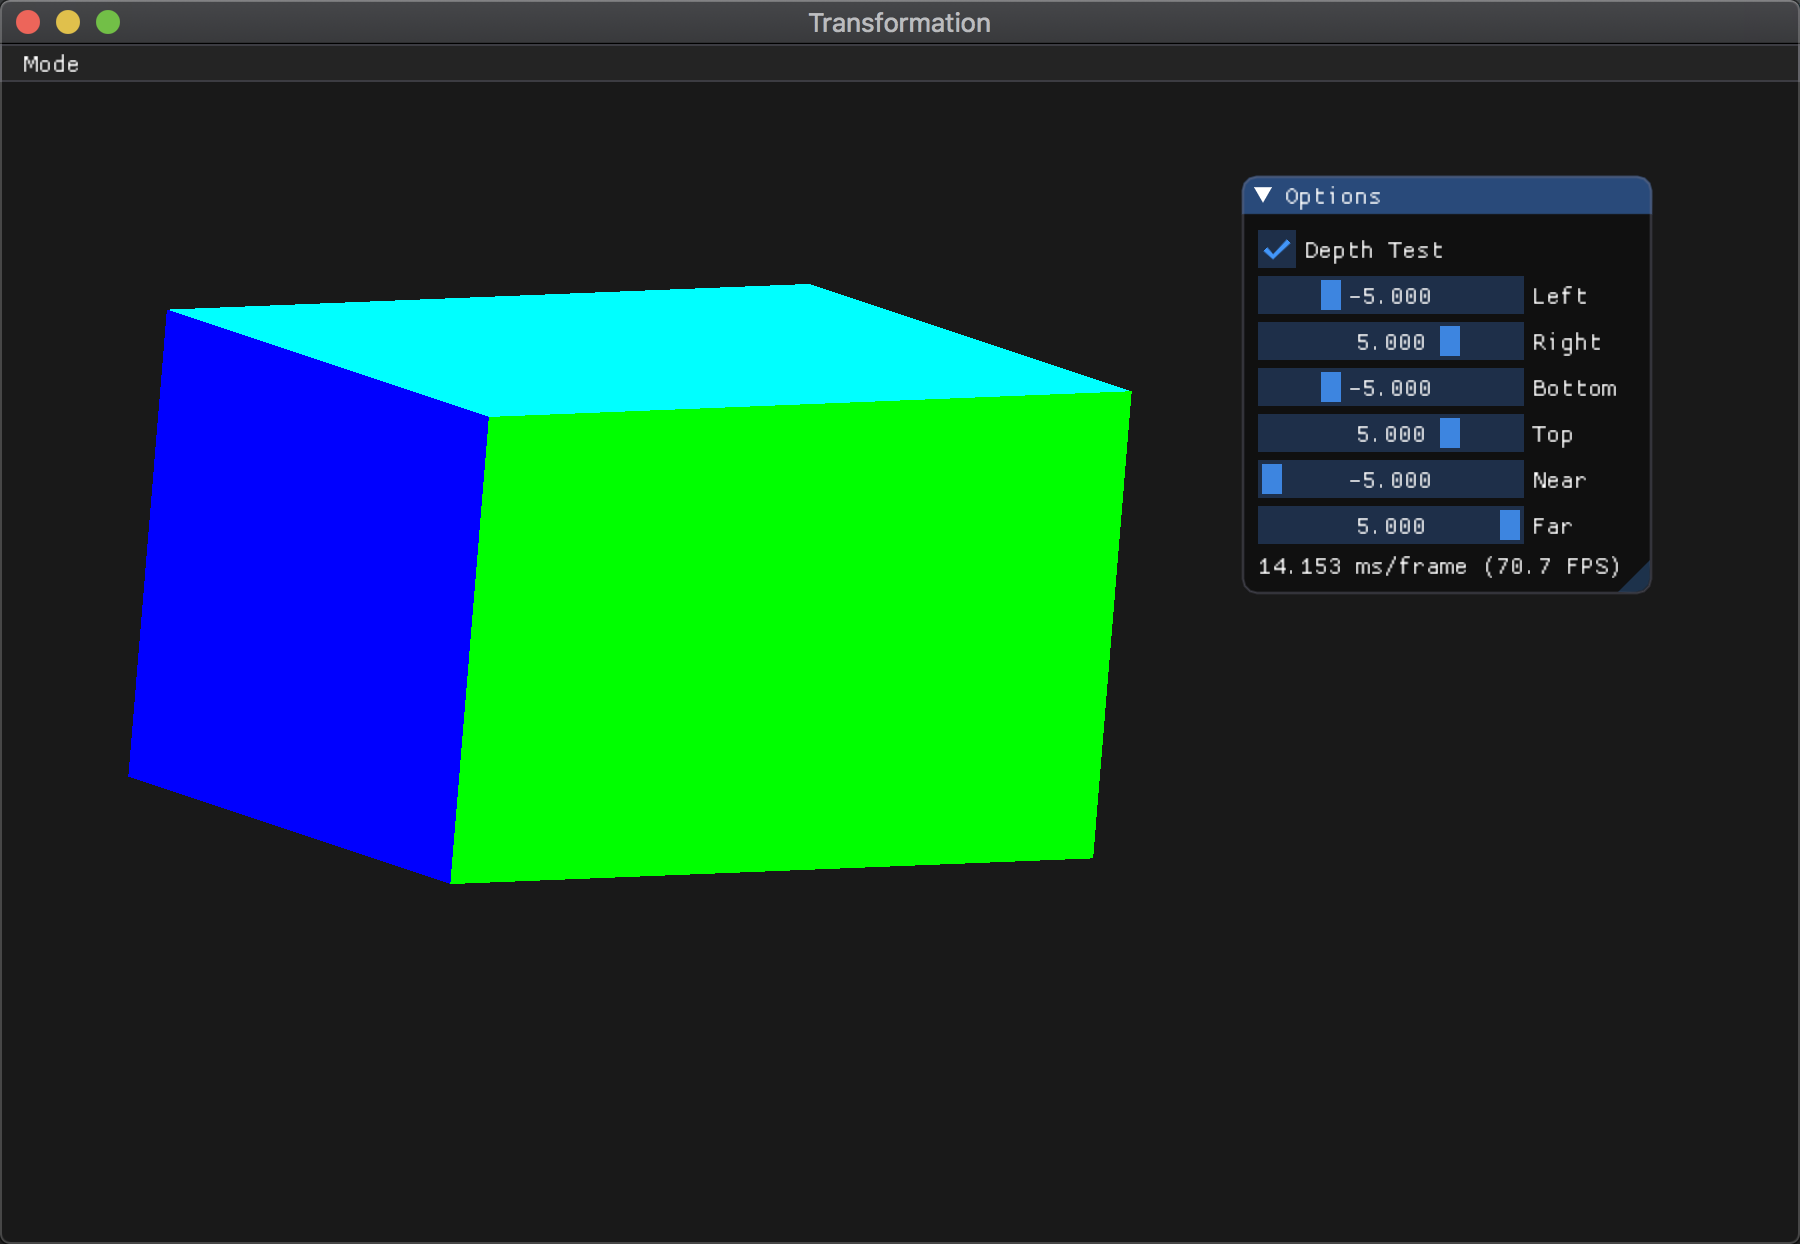
\includegraphics[scale=0.35]{ortho_1.png}
        \end{center}

        通过 left, right, bottom和 top 参数可以调整平截头体的大小,从而调整坐标在屏幕中显示的效果,当调整 near 和 far 参数时在近平面前和远平面后的所有坐标将被裁剪,如图:
        \begin{center}
            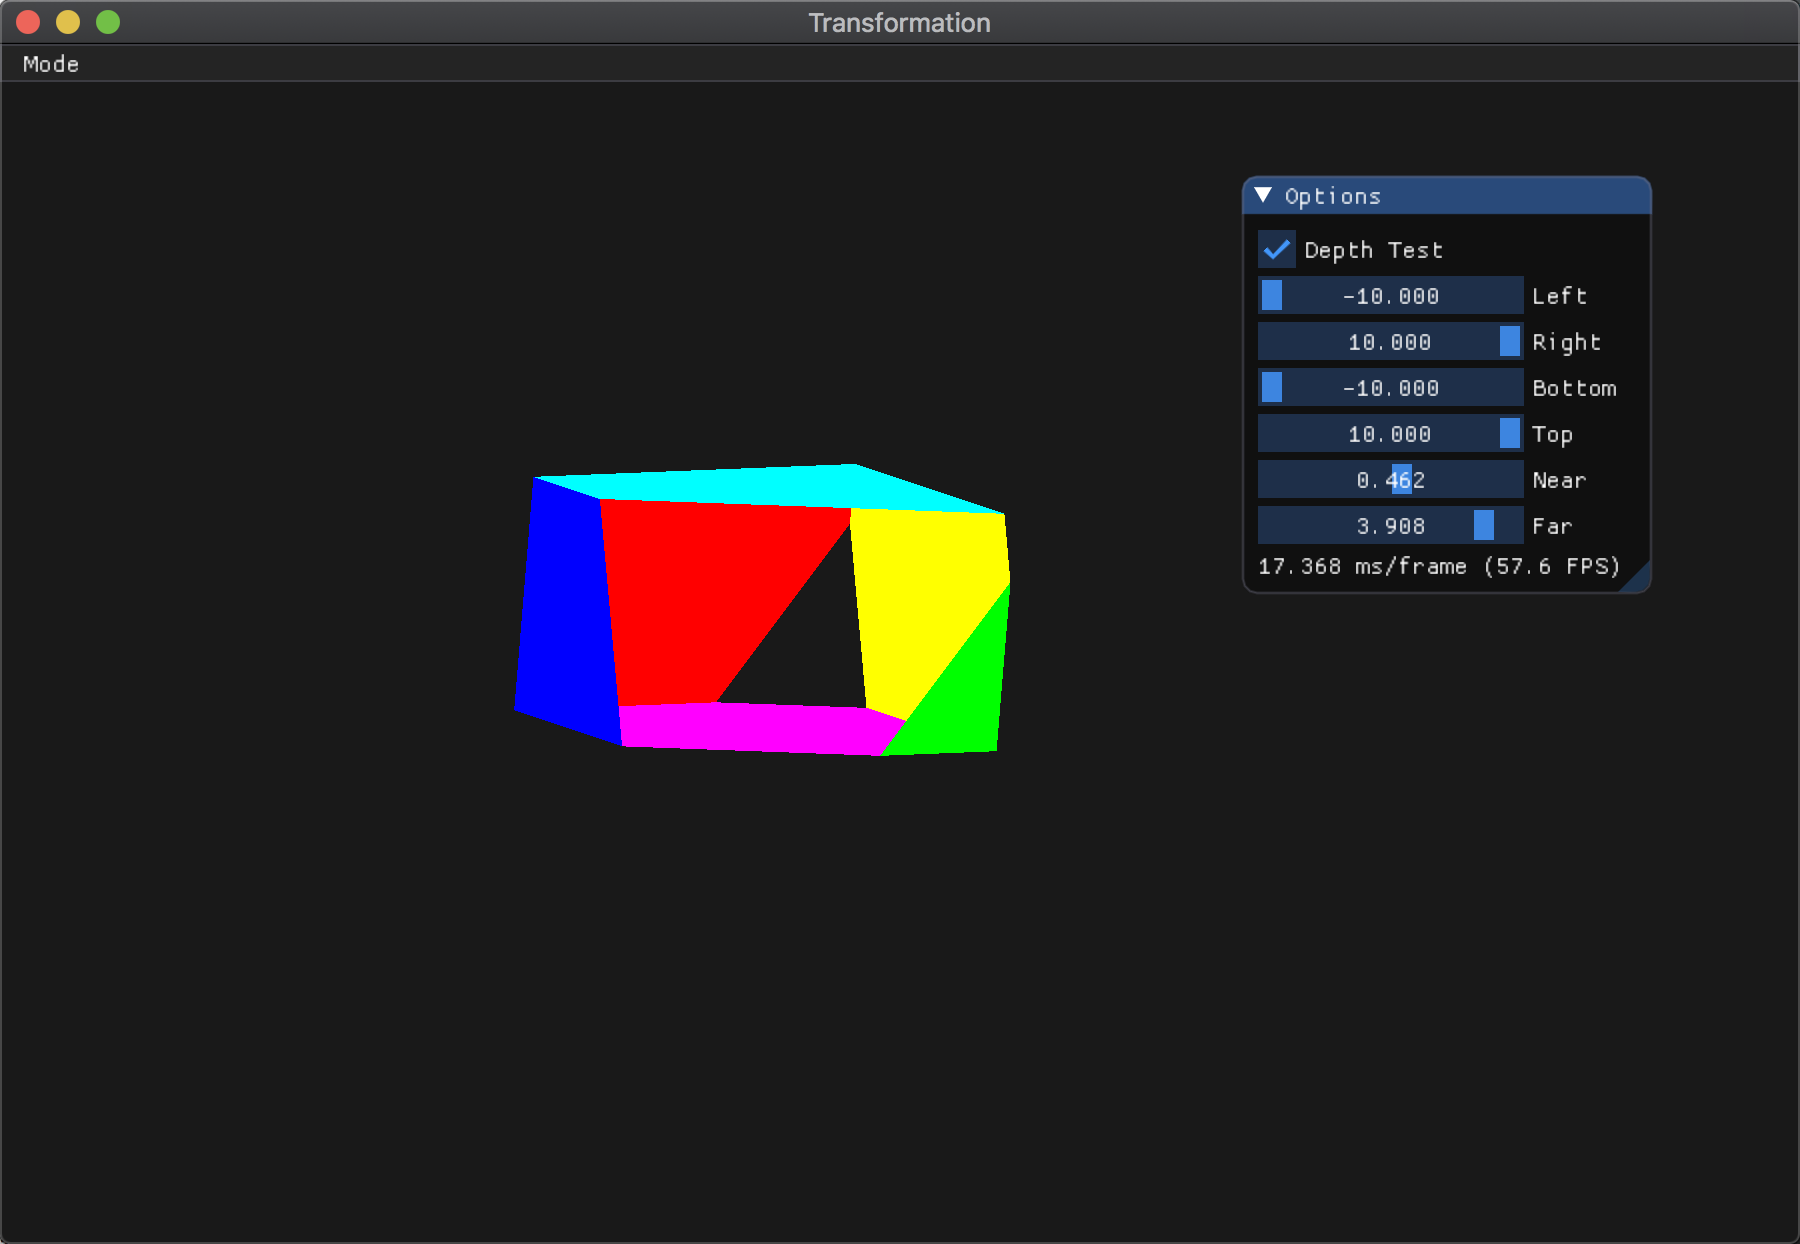
\includegraphics[scale=0.35]{ortho_2.png}
        \end{center}

        \item 透视投影(perspective projection):实现透视投影,使用多组参数,比较结果差异
        
        透视投影使用了如下的平截头体进行裁剪:
        \begin{center}
            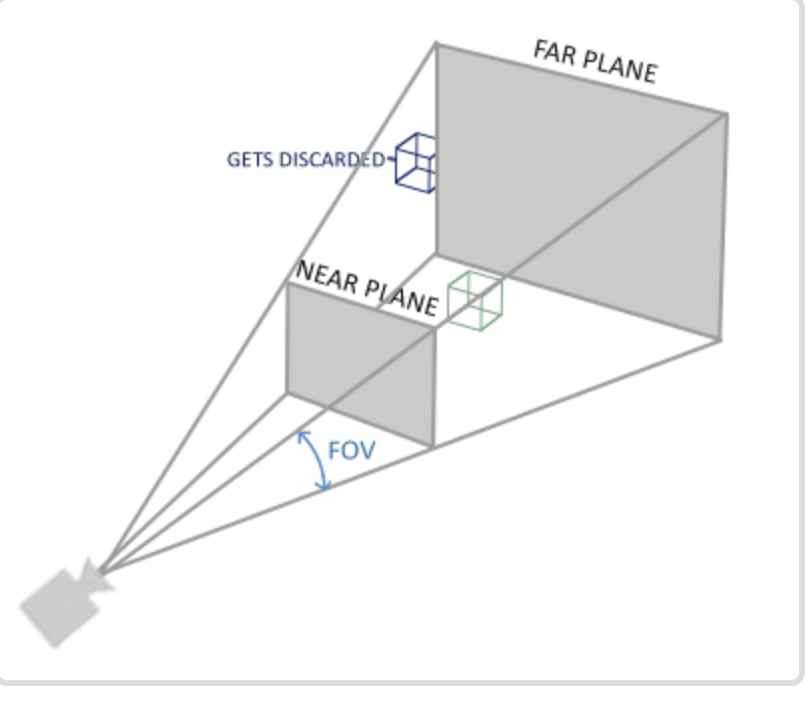
\includegraphics[scale=0.6]{persp_img.png}
        \end{center}
        在 GLM 中透视投影的函数如下:
        \begin{lstlisting}
    detail::tmat4x4<T> glm::gtc::matrix_transform::perspective 	( 	
        T const &  	fovy,
		T const &  	aspect,
		T const &  	zNear,
		T const &  	zFar 
	) 		
        \end{lstlisting}
        
        fovy参数指的是视野,aspect 参数为宽高比,一般设为视口的宽除以高,zNear 和 zFar 参数为近平面和远平面的距离.
        获得的效果如下:
        \begin{center}
            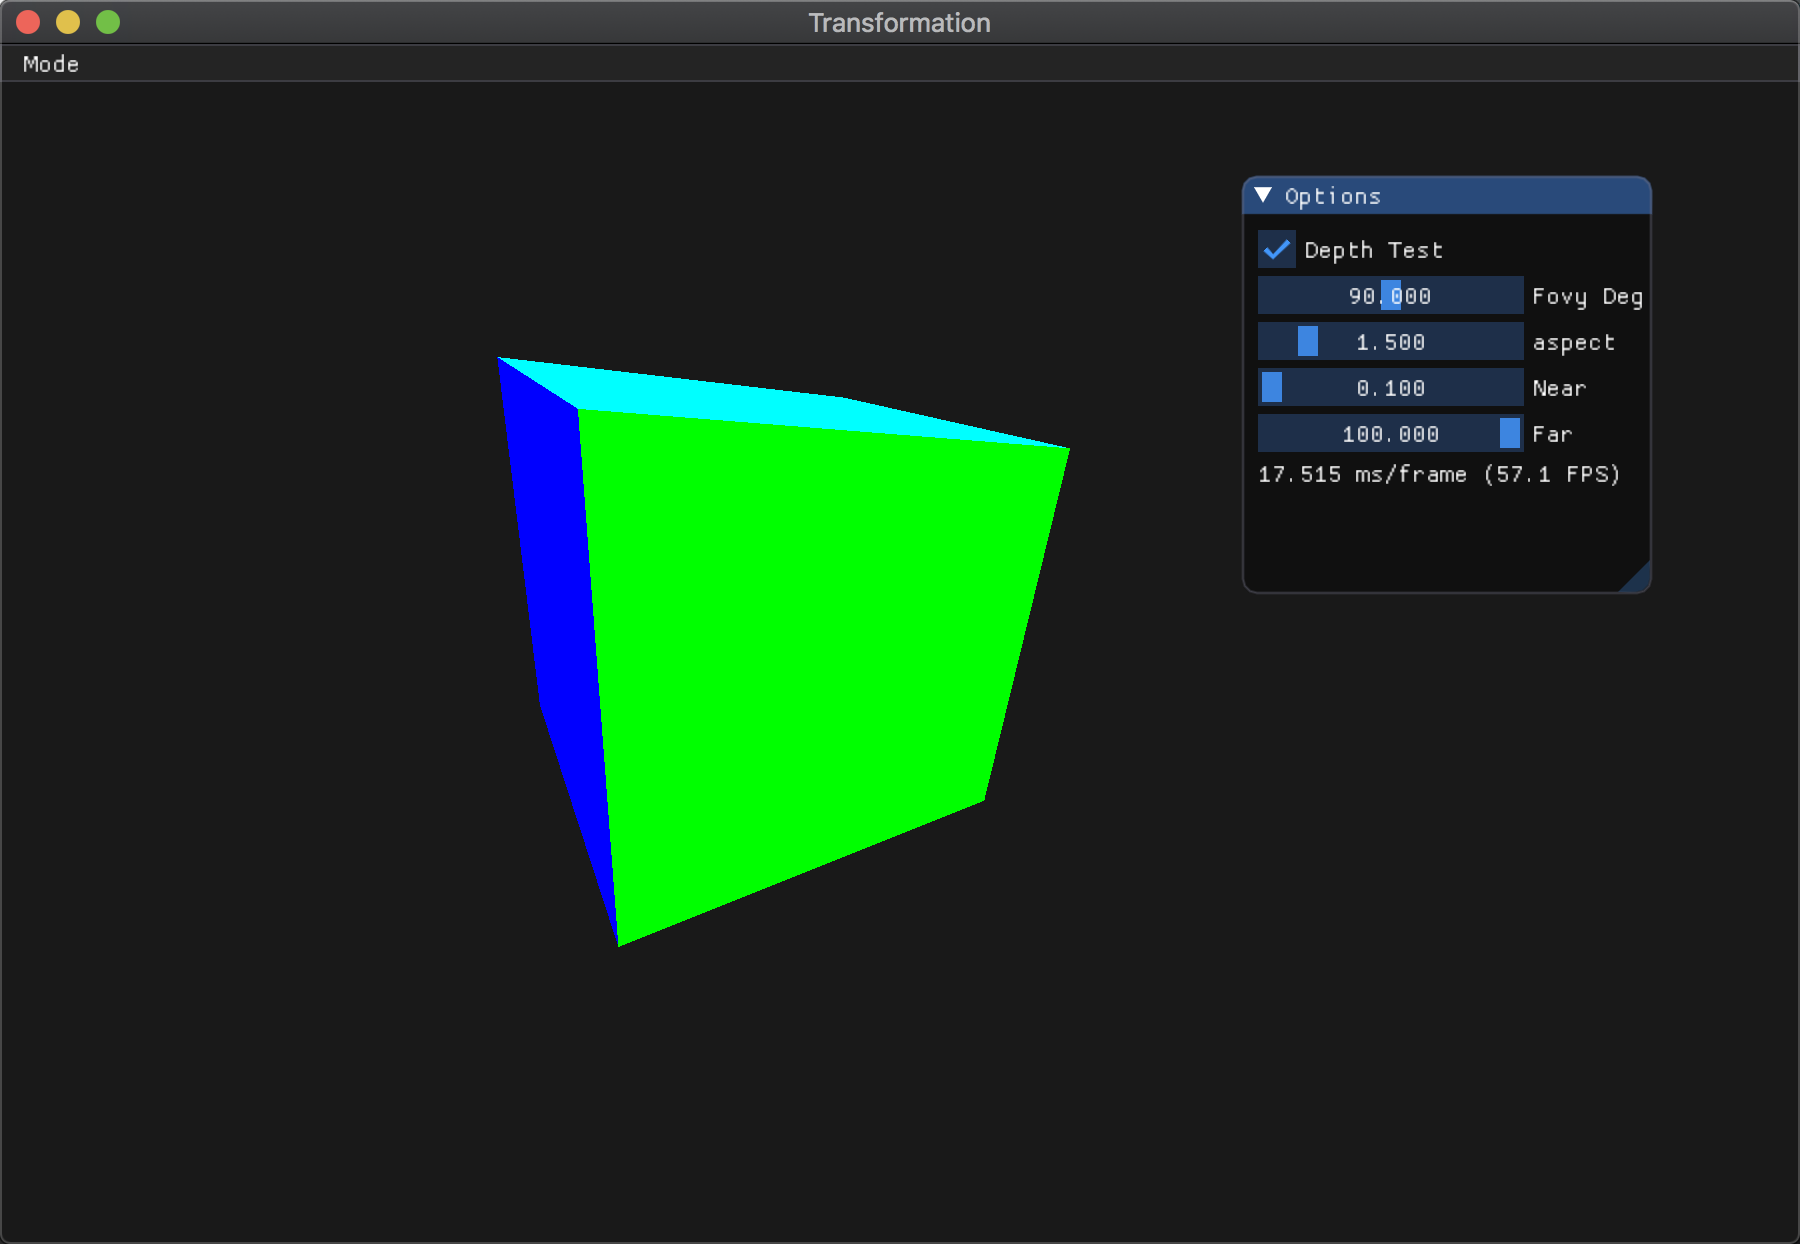
\includegraphics[scale=0.35]{persp_1.png}
        \end{center}
        通过调整 fovy 可以 设置观察空间大小,调整 aspect 可以控制观察空间的比例,调整 near 和 far 可以对两平面之外的坐标进行裁剪。如图:
        \begin{center}
            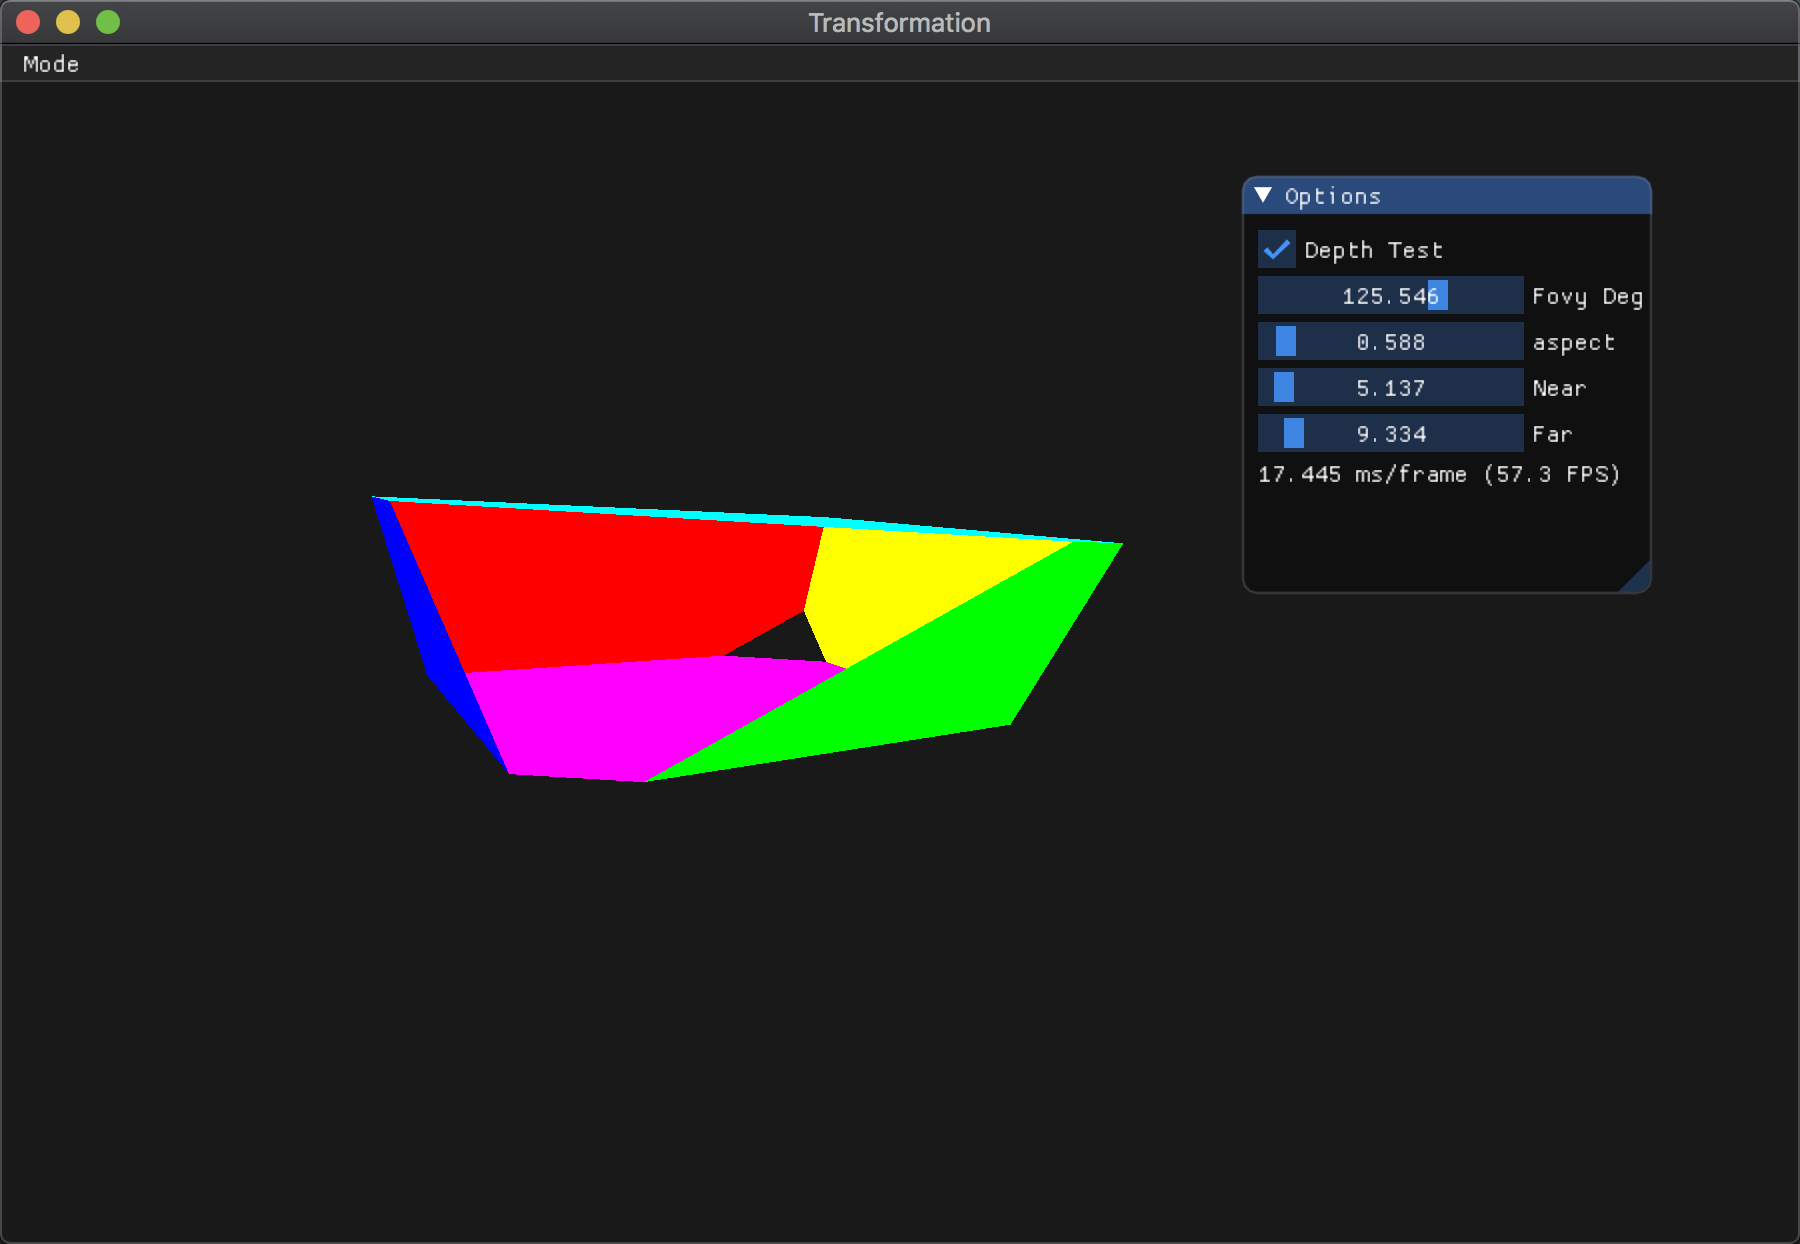
\includegraphics[scale=0.35]{persp_2.png}
        \end{center}
    \end{enumerate}
    \item 视角变换(View Changing):把cube放置在(0, 0, 0)处,做透视投影,使摄像机围绕cube旋转,并且时刻看着cube中心
    
    令摄像机围绕 cube 旋转的方法是根据时间调整摄像机的位置,调整方法如下:
    \begin{equation}
        \begin{aligned}
            x = r\sin t \\
            z = r\cos t
        \end{aligned}
    \end{equation}

    由于$x^2+z^2=r^2$,因此摄像机将以 r 为半径围绕 cube 旋转。控制摄像机位置的方法如下:
    \begin{lstlisting}
        float cam_1 = sin(glfwGetTime()) * radius;
        float cam_2 = cos(glfwGetTime()) * radius;
        camera_pos = glm::vec3(0, cam_1, cam_2);
        up = glm::vec3(0, cam_2 > 0 ? 1: -1, 0);
        view *= glm::lookAt(camera_pos,
                        glm::vec3(0.0f, 0.0f, 0.0f),
                        up);
    \end{lstlisting}
    以上方法中摄像机绕 y 轴旋转,通过调整上向量和位置,也可以令摄像机绕x 轴或 z 轴旋转。
    
    旋转中的效果如下:
    \begin{center}
        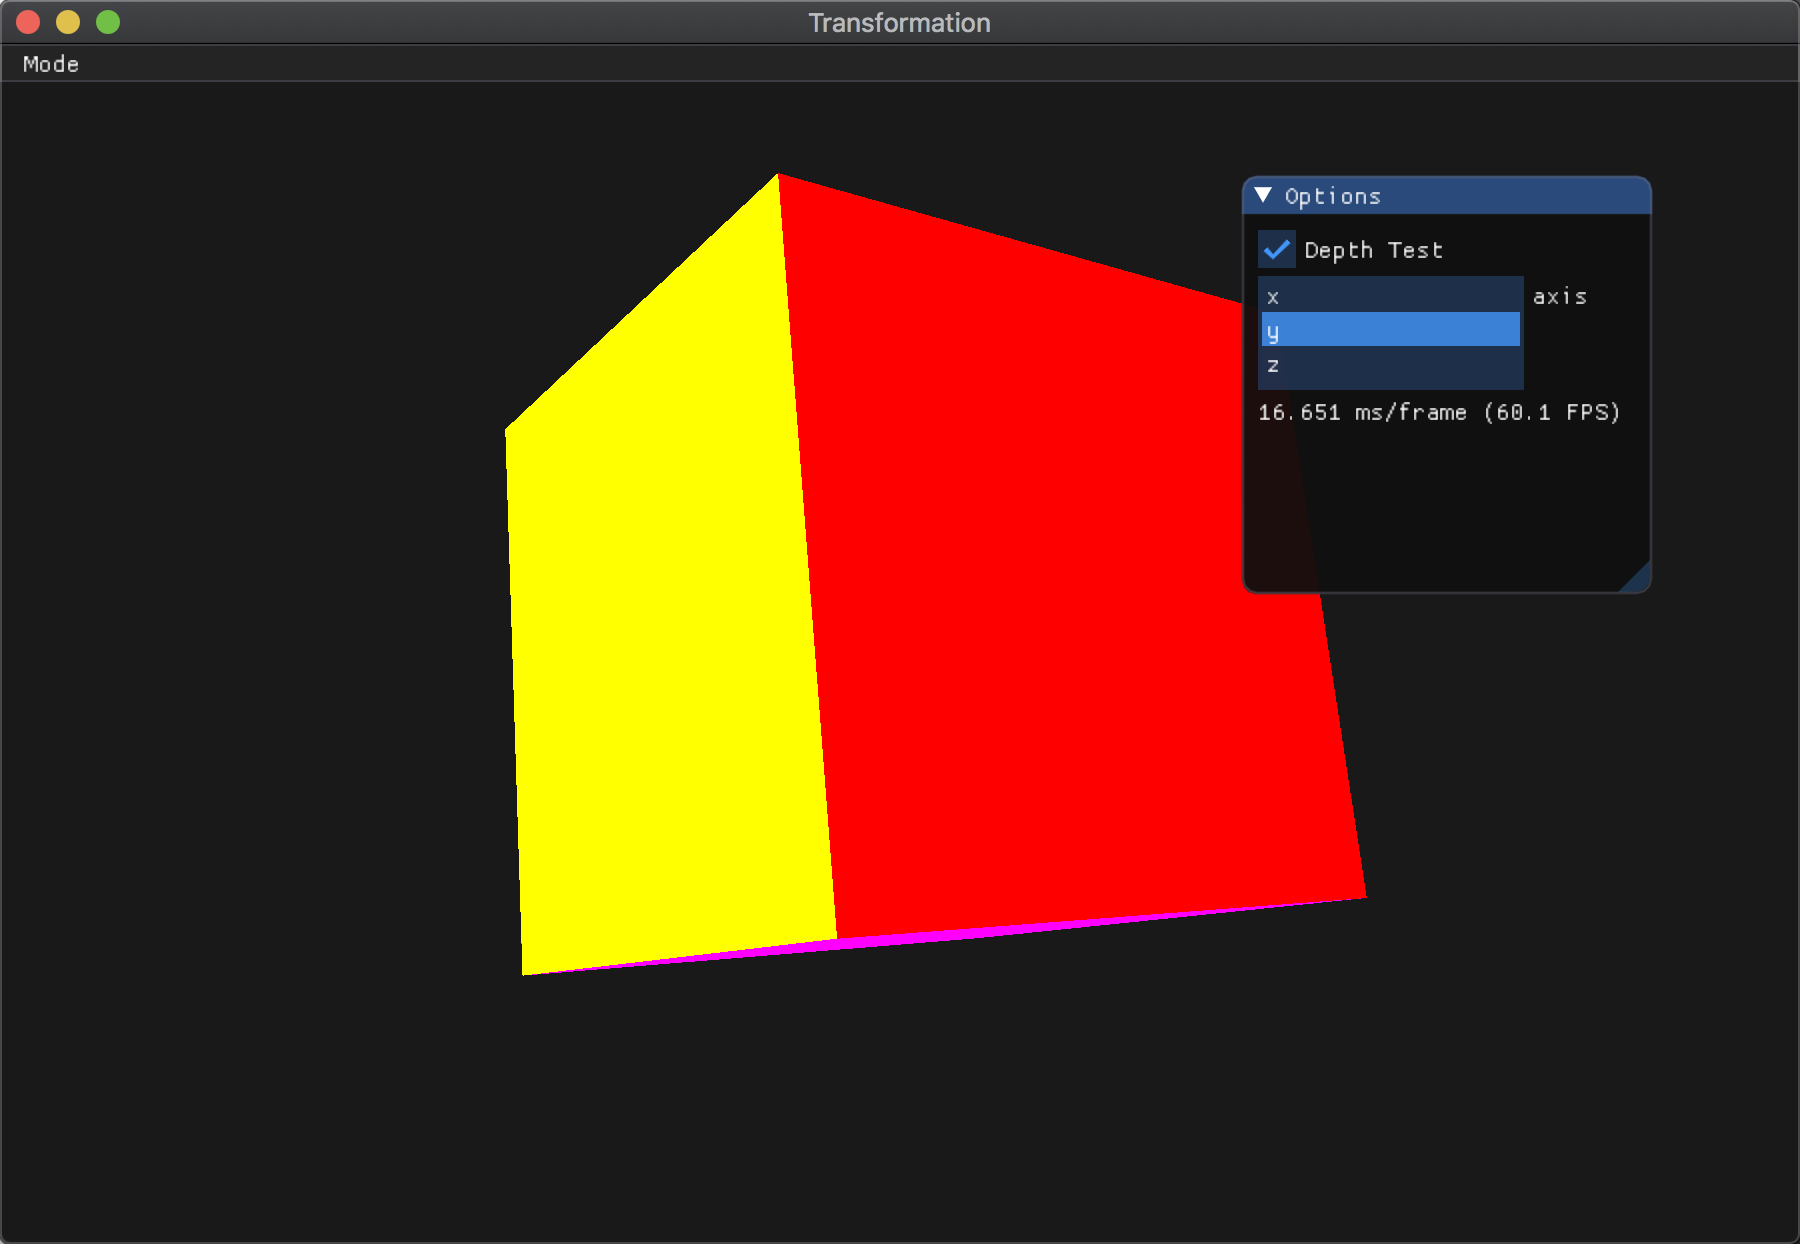
\includegraphics[scale=0.35]{rotate.png}
    \end{center}

    \item 在现实生活中,我们一般将摄像机摆放的空间View matrix和被拍摄的物体摆设的空间Model matrix分开,但 是在OpenGL中却将两个合二为一设为ModelView matrix,通过上面的作业启发,你认为是为什么呢?在报 告中写入。(Hints:你可能有不止一个摄像机)
    
    在先前版本使用固定管线的 OpenGL 中,提供了单独的 projection matrix, 但仅提供了结合 model 和 view 的 ModelView Matrix, 原因可能如下:
    \begin{enumerate}
        \item 结合 model 和 view 可以减少着色器中对每一个顶点进行的矩阵相乘操作,仅需在 CPU 中进行一次对矩阵的计算,在顶点数较多的情况下可以提升性能
        \item model 矩阵将顶点从局部坐标转为世界坐标,而世界坐标下进行数值计算对于数值较大的顶点可能会出现一定的误差,通过 view 矩阵将其转换到观察空间(摄像机)后可以使这些顶点距离更近,降低计算误差。
        \item model和 view 矩阵都是通过对物体进行位移、旋转、缩放等来将物体变换到不同的空间,因此可将其二合一,而投影矩阵则是对范围内的坐标进行变换以映射到设备坐标范围内,并对屏幕外的坐标进行裁剪。
    \end{enumerate}
\end{enumerate}

\section{Bonus}
实现一个camera类,当键盘输入 w,a,s,d,能够前后左右移动;当移动鼠标,能够视角移动("look around"), 即类似FPS(First Person Shooting)的游戏场景。

实现的 Camera 类中包含了摄像机位置,摄像机方向,摄像机右向量,摄像机上向量四个向量,以及透视投影的参数。构建摄像机对象时需要传入一个\lstinline{GLFWWindow*}以便摄像机获取键盘和鼠标输入信息进行移动。摄像机也提供了对移动速度和鼠标灵敏度的调整。摄像机的所有者可以通过调用\lstinline{getViewMatrix}和\lstinline{getProjectionMatrix}获得 View 和 projection 矩阵。

读取键盘和鼠标输入用的是\lstinline{glfwGetKey}和\lstinline{glfwGetCursorPos}函数,根据键盘按下哪个键决定向哪个方向移动(改变摄像机位置),按下 ESC 键时则退出鼠标模式,鼠标则根据与上一次位置的偏差对欧拉角进行更改(改变摄像机方向)。

欧拉角由yaw, pitch和 roll 三个角组成,分别代表3D 空间中旋转的三个值。在本次摄像机中不需要使用 roll 的值,将 yaw 和 pitch 转为摄像机方向的方法为:
\begin{equation}
    \begin{aligned}
        y=\sin (pitch)\\
        x=\cos (pitch)\times \cos (yaw)\\
        z=\cos (pitch)\times \sin (yaw)
    \end{aligned}
\end{equation}

移动至 cube 内部的效果如下图(移动鼠标和操作键盘的动态效果请见 demo):
\begin{center}
    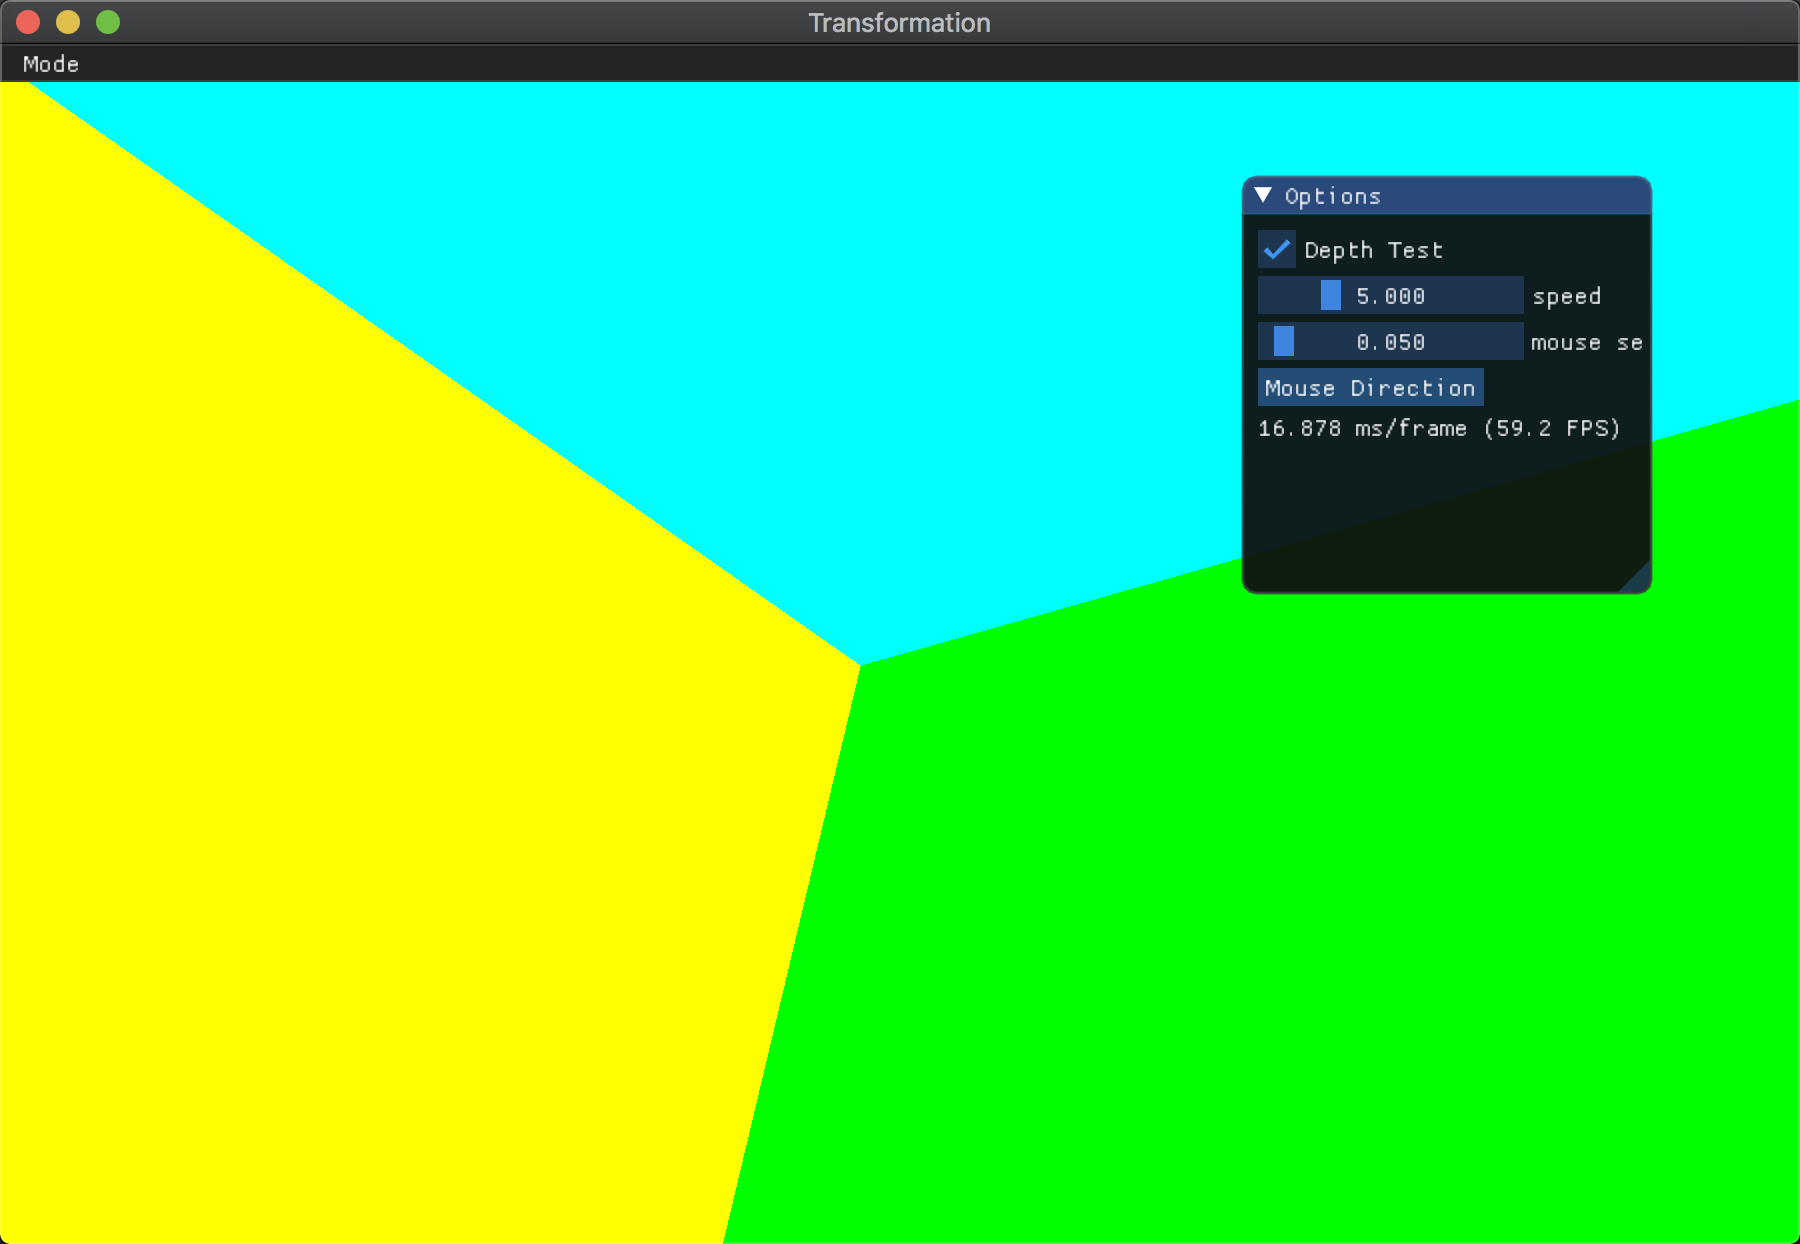
\includegraphics[scale=0.35]{camera.png}
\end{center}
\end{document}
\grid
\grid
